% NeurAps — Insight 2.0 Grand Finale, Part 3: Technical Procedure (Beamer)
% Build: pdflatex neuraps_technical.tex  (run twice)
\documentclass[aspectratio=169,10pt]{beamer}

\usepackage[T1]{fontenc}
\usepackage{libertine}
\usepackage{booktabs}
\usepackage{tikz}
\usetikzlibrary{positioning}

% ---------- palette (identical to the main deck) ----------
\definecolor{navy}{HTML}{1F3A5F}
\definecolor{burg}{HTML}{8C2F2F}
\definecolor{ink}{HTML}{1A1A1A}
\definecolor{mutedgray}{HTML}{555F66}
\definecolor{lightbg}{HTML}{F2F5F8}
\definecolor{ruleline}{HTML}{D6DBE0}

\usetheme{default}
\definecolor{paper}{HTML}{FCFCFA}
\definecolor{navyfaint}{HTML}{2C4A73}
\setbeamercolor{background canvas}{bg=paper}
\setbeamercolor{structure}{fg=navy}
\setbeamercolor{frametitle}{fg=navy,bg=paper}
\setbeamercolor{title}{fg=white}
\setbeamercolor{normal text}{fg=ink}
\setbeamercolor{alerted text}{fg=burg}
\setbeamercolor{block title}{fg=paper,bg=navy}
\setbeamercolor{block body}{fg=ink,bg=lightbg}
\setbeamercolor{block title alerted}{fg=paper,bg=burg}
\setbeamercolor{block body alerted}{fg=ink,bg=lightbg}
\setbeamertemplate{navigation symbols}{}
\setbeamertemplate{blocks}[rounded]
\setbeamertemplate{itemize item}{\tikz{\fill[burg] (0,0) rectangle (0.55ex,0.55ex);}}
\setbeamertemplate{itemize subitem}{\tikz{\draw[navy,thick] (0,0) rectangle (0.5ex,0.5ex);}}
\setbeamerfont{frametitle}{series=\bfseries,size=\LARGE}
\setbeamersize{text margin left=1.05cm,text margin right=1.05cm}

\setbeamertemplate{frametitle}{%
  \vspace{0.55cm}%
  {\usebeamerfont{frametitle}\usebeamercolor[fg]{frametitle}\insertframetitle}\par
  \vspace{0.12cm}{\color{burg}\rule{1.35cm}{2.6pt}}\par\vspace{0.1cm}}

\setbeamertemplate{footline}{%
  \begin{tikzpicture}[baseline]
    \fill[ruleline] (0,0) rectangle (\paperwidth,0.55mm);
    \pgfmathsetmacro{\prog}{\insertframenumber/\inserttotalframenumber*\paperwidth/1cm}
    \fill[burg] (0,0) rectangle (\prog cm,0.55mm);
  \end{tikzpicture}\par\vspace{1.4pt}%
  \hspace{1.05cm}{\tiny\color{mutedgray}Insight 2.0 --- Datathon 2026 \;·\; Team NeurAps \;·\; Technical procedure}%
  \hfill{\tiny\color{mutedgray}\insertframenumber\,/\,\inserttotalframenumber}\hspace{1.05cm}\vspace{3.5pt}}

\setbeamertemplate{section page}{%
  \begin{tikzpicture}[remember picture,overlay]
    \fill[navy] (current page.south west) rectangle (current page.north east);
    \node[anchor=south east,color=navyfaint,font=\fontsize{130}{130}\selectfont\bfseries,
          inner sep=0pt,opacity=0.85] at ([xshift=-0.4cm,yshift=0.2cm]current page.south east)
          {\insertsectionnumber};
    \node[anchor=west,color=white,font=\huge\bfseries,text width=0.8\paperwidth,align=left]
          at ([xshift=1.2cm,yshift=0.3cm]current page.west) {\insertsection};
    \draw[burg,line width=3pt] ([xshift=1.2cm,yshift=1.35cm]current page.west) -- ++(1.35,0);
    \node[anchor=west,color=ruleline,font=\small]
          at ([xshift=1.2cm,yshift=1.85cm]current page.west) {Part 3 \;·\; Section \insertsectionnumber};
  \end{tikzpicture}}
\AtBeginSection[]{\begin{frame}[plain]\sectionpage\end{frame}}

\newcommand{\code}[1]{{\ttfamily #1}}
\newcommand{\file}[1]{{\ttfamily\footnotesize\color{navy}#1}}

\begin{document}

% ---------- 1 title ----------
\begin{frame}[plain]
  \begin{tikzpicture}[remember picture,overlay]
    \fill[navy] (current page.south west) rectangle (current page.north east);
    \fill[burg] (current page.north west) rectangle ([yshift=-0.16cm]current page.north east);
    \node[anchor=west,color=ruleline,font=\footnotesize\ttfamily]
      at ([xshift=1.2cm,yshift=-1.5cm]current page.north west)
      {INSIGHT 2.0 --- GRAND FINALE \;·\; PART 3 OF 3};
    \node[anchor=west,color=white,font=\LARGE\bfseries,text width=0.86\paperwidth,align=left]
      at ([xshift=1.2cm,yshift=0.9cm]current page.west)
      {Technical Procedure\\[4pt]
       {\large\mdseries\color{ruleline}Workflow \;·\; Methodology \;·\; Reproducibility}};
    \draw[burg,line width=3pt] ([xshift=1.2cm,yshift=2.1cm]current page.west) -- ++(1.35,0);
    \node[anchor=west,color=ruleline,font=\large]
      at ([xshift=1.2cm,yshift=-0.6cm]current page.west)
      {\textbf{\color{white}Team NeurAps} \;·\; 5 September 2026};
    \node[anchor=west,color=ruleline,font=\small,text width=0.8\paperwidth]
      at ([xshift=1.2cm,yshift=-2.0cm]current page.west)
      {Everything shown here is a file in our repository or a cell in the submitted notebook.
       Ask us to open any of them.};
  \end{tikzpicture}
\end{frame}

\section{Workflow}

\begin{frame}{The loop we ran, end to end, for every idea}
  \centering
  \resizebox{\textwidth}{!}{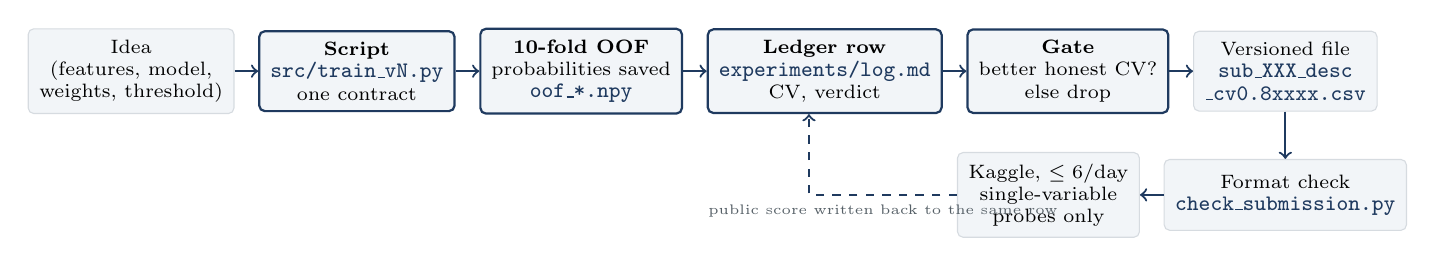
\begin{tikzpicture}[
    node distance=3mm,
    st/.style={draw=navy,thick,fill=lightbg,rounded corners=2pt,align=center,font=\scriptsize,
               minimum height=9mm,inner sep=4pt},
    pl/.style={draw=ruleline,fill=lightbg,rounded corners=2pt,align=center,font=\scriptsize,
               minimum height=9mm,inner sep=4pt},
    arr/.style={->,thick,navy}]
    \node[pl] (a) {Idea\\(features, model,\\weights, threshold)};
    \node[st,right=of a] (b) {\textbf{Script}\\\file{src/train\_vN.py}\\one contract};
    \node[st,right=of b] (c) {\textbf{10-fold OOF}\\probabilities saved\\\file{oof\_*.npy}};
    \node[st,right=of c] (d) {\textbf{Ledger row}\\\file{experiments/log.md}\\CV, verdict};
    \node[st,right=of d] (e) {\textbf{Gate}\\better honest CV?\\else \alert{drop}};
    \node[pl,right=of e] (f) {Versioned file\\\file{sub\_XXX\_desc}\\\file{\_cv0.8xxxx.csv}};
    \draw[arr] (a)--(b); \draw[arr] (b)--(c); \draw[arr] (c)--(d); \draw[arr] (d)--(e); \draw[arr] (e)--(f);
    \node[pl,below=6mm of f] (g) {Format check\\\file{check\_submission.py}};
    \node[pl,left=of g] (h) {Kaggle, $\le 6$/day\\single-variable\\probes only};
    \draw[arr] (f)--(g); \draw[arr] (g)--(h);
    \draw[arr,dashed] (h.west) -| ([xshift=-2mm]d.south) node[pos=0.25,below,font=\tiny,color=mutedgray]{public score written back to the same row};
  \end{tikzpicture}}
  \vspace{3pt}
  \begin{columns}[t]
    \column{.5\textwidth}\tiny
    \textbf{Rules the loop enforced}
    \begin{itemize}\tiny
      \item \file{data/raw/} is never modified; derived artifacts go to \file{data/processed/}.
      \item One shared \code{build\_features()} is the single source of truth for every model.
      \item Every script prints per-model OOF, blend weights and the tuned threshold; nothing is judged by eye.
      \item A result is recorded before the next idea starts; drops are rows, not deletions.
    \end{itemize}
    \column{.5\textwidth}\tiny
    \textbf{Repository layout}
    \begin{itemize}\tiny
      \item \file{src/}: one script per pipeline version, plus sweeps, tuning, stacking, checks
      \item \file{data/processed/}: the component bank --- OOF and test probabilities for every model trained
      \item \file{submissions/}: 30 versioned files, 23 sent to the leaderboard
      \item \file{experiments/log.md}, \file{memory/insights.md}, \file{notebooks/}: ledger, findings, the reproducible solution
    \end{itemize}
  \end{columns}
\end{frame}

\begin{frame}{The ledger: what a row looks like}
  \scriptsize
  Every experiment, kept or dropped, is one row. Three real rows:
  \vspace{4pt}
  \begin{tabular}{@{}p{0.45cm}p{3.9cm}p{3.4cm}p{1.4cm}p{3.1cm}@{}}
    \toprule
    \# & Change & CV (OOF weighted F1) & Public & Verdict\\
    \midrule
    2 & Engineered features + LGBM/XGB/CatBoost blend, threshold 0.59 & 0.87768 (lgb .87704 / xgb .87672 / cat .87721) & 0.876023 & keep --- CV $+0.0007$ gave LB $+0.0017$\\
    3 & Optuna-tuned LGBM + XGB + Cat, 10-fold $\times$ 3 seeds, threshold 0.56 & 0.87964 & 0.875246 & CV$\leftrightarrow$LB diverged; probe the threshold next\\
    17 & RF/ET/MLP diversity: v4 + 5\% each, threshold 0.575 & 0.87996 (split-half: .87934 vs .87876 $\Rightarrow$ real $+0.0006$) & 0.875506 & best honest CV --- final pick candidate\\
    \bottomrule
  \end{tabular}
  \vspace{8pt}
  \begin{block}{Why the ledger mattered technically}
    The endgame question --- ``which two files?'' --- was answered by sorting this table on the honest-CV column,
    not by memory. The public column exists in the same row so that CV$\leftrightarrow$LB gaps are visible per experiment.
  \end{block}
\end{frame}

\section{Methodology}

\begin{frame}{Feature construction in code}
  \scriptsize
  \begin{tabular}{@{}p{3.1cm}p{9.6cm}@{}}
    \toprule
    \textbf{Step} & \textbf{Implementation}\\
    \midrule
    Sentinel decoding & \code{pd.to\_numeric(col, errors="coerce")}; any value $\ge 990$ set to missing
      (999 / 998 are ``unknown'' codes, ``Blank(s)'' and ``Unknown or size unreasonable'' become NaN)\\
    Tumor size coalesce & \code{summary.fillna(overtime).fillna(cs\_2004\_2015)} + \code{size\_missing\_all} flag\\
    Ordinal maps & T: T0/Tis$\to$0, T1mi/T1a$\to$1, T1b$\to$1.5, T1c$\to$2, T2a$\to$2.5, T2b$\to$3, T3$\to$4, T4$\to$5;
      N0--N3$\to$0--3; M0$\to$0, M1a$\to$1, M1b$\to$2, M1c$\to$3; grade I--IV$\to$1--4; stage L/R/D$\to$1--3\\
    Composite & \code{tnm\_sum = t + n + 2*m}, unknowns filled with scale midpoints (2.5, 1.5, 1.5)\\
    Counts and flags & \code{mets\_count} (Yes across bone/brain/liver/lung), \code{mets\_known}, \code{surgery\_done},
      \code{death\_cert\_only} (regex on the reason column), \code{radiation\_given}, \code{any\_treatment}, \code{multiple\_primaries}\\
    Ratios and time & \code{nodes\_ratio = positive / max(examined, 1)} where examined $>0$; \code{years\_since\_dx = 2024 - year}\\
    Categoricals & pandas \code{category} with levels unioned over train and test
      (\code{union\_categoricals}) so every library sees identical codes\\
    Three encodings & LightGBM: native categories \;·\; XGBoost/RF/ET: integer codes \;·\; CatBoost/MLP: strings with an explicit ``NA'' level\\
    \bottomrule
  \end{tabular}
  \vspace{4pt}\par\tiny\color{mutedgray}
  35 raw predictors $\to$ 53 model columns. No target statistics outside a fold; nothing fitted on test.
\end{frame}

\begin{frame}{Validation protocol, as implemented}
  \begin{columns}[t]
    \column{.52\textwidth}\footnotesize
    \begin{itemize}\footnotesize
      \item \code{StratifiedKFold(10, shuffle=True, random\_state=seed)}, seeds 42 / 2026 / 7.
      \item Each fold: train on 9 parts (+ pseudo-rows), early-stop on the 10th, predict the 10th
            $\Rightarrow$ one out-of-fold probability per training patient.
      \item OOF averaged over seeds; test probability averaged over all fold models $\times$ seeds.
            No refit on the full set: the fold models are early-stopped, and averaging them is a free ensemble.
      \item Threshold: sweep 0.35--0.75 in steps of 0.005 on pooled OOF. Report the global argmax
            \emph{and} the median of per-fold optima; when they disagree, the score is fragile.
    \end{itemize}
    \column{.48\textwidth}\footnotesize
    \begin{block}{Split-half verification (pseudo-code)}\scriptsize
      \code{A, B = random halves of OOF rows}\\
      \code{choice = argmax over candidates of score(A)}\\
      \code{report score(B) for that frozen choice}\\
      \code{compare with score(B) of the incumbent}
    \end{block}
    \begin{alertblock}{What it decided}\scriptsize
      Diversity mixture: survived ($+0.0006$). Per-year thresholds: failed. Distillation: never passed
      (mechanism leaked). Stacking: no gain.
    \end{alertblock}
  \end{columns}
\end{frame}

\begin{frame}{Model configurations, exactly}
  \scriptsize
  \begin{tabular}{@{}p{2.2cm}p{7.6cm}p{2.9cm}@{}}
    \toprule
    \textbf{Model} & \textbf{Parameters} & \textbf{Input encoding}\\
    \midrule
    LightGBM (both stages) & lr 0.05, num\_leaves 27, min\_data\_in\_leaf 20, feature\_fraction 0.40, bagging\_fraction 0.60 (freq 1),
      $\lambda_1$ 7.36, $\lambda_2$ 0.078, min\_gain\_to\_split 0.19; $\le 3000$ rounds, early stopping 100 & native categoricals\\
    XGBoost & lr 0.05, max\_depth 7, subsample 0.8, colsample\_bytree 0.8, min\_child\_weight 10; log-loss early stopping 100 & integer codes\\
    CatBoost & lr 0.05, depth 7, l2\_leaf\_reg 5; Logloss early stopping 100; ordered target statistics & strings + ``NA''\\
    RandomForest / ExtraTrees & 800 trees, min\_samples\_leaf 5, max\_features $\sqrt{p}$ & integer codes, median impute\\
    MLP & layers 128$\to$64 ReLU, $\alpha$ 1e-3, batch 512, $\le 60$ epochs, early stopping (patience 8) & one-hot (min freq 20) + standardised numerics\\
    \midrule
    Optuna study & 40 trials, TPE sampler, 5-fold; objective = mean per-fold best-threshold weighted F1;
      space: leaves 15--255, min\_data 10--200, feature/bagging fractions, $\lambda_1$, $\lambda_2$, min\_gain & LightGBM only\\
    \bottomrule
  \end{tabular}
  \vspace{5pt}\par\tiny\color{mutedgray}
  The tuned LightGBM parameters are hard-coded in the notebook and used in both stages. XGBoost and CatBoost were never tuned;
  our controlled probe showed no leaderboard gain from tuning, so no further budget went there.
\end{frame}

\begin{frame}{Blend, mixture and decision threshold}
  \begin{columns}[t]
    \column{.5\textwidth}\small
    \textbf{GBM blend weights}
    \begin{itemize}\small
      \item Objective: $-\max_t\,\mathrm{wF1}\big(y,\; \textstyle\sum_m w_m\,p_m > t\big)$ on OOF.
      \item Optimiser: Nelder--Mead (derivative-free simplex), because thresholded F1 is a step function.
      \item $w \leftarrow |w| / \sum|w|$; solutions landed near $1/3$ each (e.g.\ 0.344 / 0.333 / 0.323).
    \end{itemize}
    \textbf{Final probability}
    \[ p = 0.85\,p_{\text{GBM}} + 0.05\,(p_{\text{RF}} + p_{\text{ET}} + p_{\text{MLP}}) \]
    \column{.5\textwidth}\small
    \textbf{Decision}
    \begin{itemize}\small
      \item Sweep on pooled OOF $\Rightarrow$ 0.575; per-fold optima 0.570--0.575.
      \item Label Dead iff $p > 0.575$. Predicted Dead rate 85.8\% (train 83.0\%).
      \item OOF at 0.575: weighted F1 0.87996; at 0.5: 0.87518. Accuracy is 88.4\% at both cuts ---
            only the metric moves.
    \end{itemize}
    \begin{block}{Duplicate correction}\scriptsize
      283 test rows are exact 35-column copies of train rows; they take the train label. Changed 1 prediction.
    \end{block}
  \end{columns}
\end{frame}

\begin{frame}[fragile]{Pseudo-labelling, inside the fold}
  \begin{columns}[t]
    \column{.5\textwidth}
    \begin{block}{The augmentation, per fold}
\begin{semiverbatim}\scriptsize
mask = (p_test > 0.99) | (p_test < 0.02)
X_ps, y_ps = X_te[mask], (p_test[mask] > .5)

for i_tr, i_va in folds:
    X_aug = concat(X[i_tr], X_ps)
    y_aug = concat(y[i_tr], y_ps)
    model.fit(X_aug, y_aug,
              eval_set=(X[i_va], y[i_va]))
    oof[i_va] += model.predict(X[i_va])
\end{semiverbatim}
    \end{block}
    \column{.5\textwidth}\small
    \begin{itemize}\small
      \item Source: stage-1 blend test probabilities. 7{,}455 rows cross (99.3\% Dead).
      \item \alert{The validation fold and the OOF array never contain a pseudo-row}; the estimate stays unbiased.
      \item Early stopping still watches only real labelled rows.
      \item Stage 2 = same trio, 10 folds $\times$ 2 seeds, retrained on the augmented folds.
      \item Tested and rejected: bands 0.05/0.97 (14{,}566 rows), and a second round from stage-2 predictions.
    \end{itemize}
  \end{columns}
\end{frame}

\section{Reproducibility}

\begin{frame}{Reproducibility checklist}
  \begin{columns}[t]
    \column{.5\textwidth}\small
    \textbf{Determinism}
    \begin{itemize}\small
      \item Fold seeds 42 / 2026 / 7; every model seeded with the fold seed; sklearn models seed 42.
      \item Tuned parameters hard-coded (no live Optuna run needed).
      \item Same \code{build\_features()} in every script and in the notebook.
    \end{itemize}
    \textbf{Environment}
    \begin{itemize}\small
      \item Python 3.12.13 \;·\; LightGBM 4.7.0 \;·\; XGBoost 3.4.1 \;·\; CatBoost 1.2.10 \;·\; scikit-learn 1.9.0 \;·\; Optuna 4.9.0 \;·\; pandas 3.0.5 \;·\; NumPy 2.5.2
      \item One Apple M2 laptop, 8 cores, 8 GB RAM, CPU only (TabPFN test used the GPU).
    \end{itemize}
    \column{.5\textwidth}\small
    \textbf{Verification}
    \begin{itemize}\small
      \item Notebook (17 cells) re-run in a clean kernel before submission.
      \item Output matches sub\_014 on \alert{36{,}000 / 36{,}000} rows; sub\_016 = sub\_014 + the one documented duplicate correction.
      \item Runtime $\approx$ 1.5 h end to end.
      \item \file{check\_submission.py} asserts: same columns, same row count, same id order, no NaN, only labels present in the sample.
      \item No external data, no manual labels, no AutoML.
    \end{itemize}
  \end{columns}
\end{frame}

\begin{frame}{Traceability: where each headline number lives}
  \scriptsize
  \begin{tabular}{@{}p{4.3cm}p{8.4cm}@{}}
    \toprule
    \textbf{Claim in Part 1} & \textbf{Where a reviewer can check it}\\
    \midrule
    OOF weighted F1 0.87996 & notebook, final-ensemble cell; ledger row 17; \file{data/processed/oof\_v4\_blend.npy} + \file{oof\_div2\_*.npy}\\
    Private 0.880410, public 0.875506 & Kaggle submission log, file \file{sub\_016\_leakfix-of-014.csv}\\
    Death rate 93.7\% $\to$ 44.4\% by year & notebook EDA cell (\code{groupby("year\_of\_diagnosis")})\\
    7{,}455 pseudo-labelled rows, 99.3\% Dead & notebook stage-2 cell; \file{src/train\_v4.py} run log\\
    Diversity $+0.0006$ (split-half) & ledger row 17; \file{src/train\_diverse2.py} OOF files\\
    Threshold 0.575 & notebook final cell (\code{best\_threshold}) and per-fold medians in \file{src/train\_v4.py}\\
    Tuned LightGBM parameters & \file{data/processed/lgb\_tuned.json}; \file{src/tune.py}\\
    283 duplicate test rows & ledger row 16; a 35-column merge of test against train\\
    Optuna, distillation, per-year thresholds rejected & ledger rows 3--4, 22, and the insights file, each with the probe submission named\\
    \bottomrule
  \end{tabular}
  \vspace{6pt}
  \begin{block}{In one sentence}
    Every number on a slide is either a printed line of a seeded script or a leaderboard entry, and the file that produced it is named.
  \end{block}
\end{frame}

% ---------- closing ----------
\begin{frame}[plain]
  \begin{tikzpicture}[remember picture,overlay]
    \fill[navy] (current page.south west) rectangle (current page.north east);
  \end{tikzpicture}
  \vspace{2.6cm}
  {\color{white}\Huge\bfseries Thank you.}\\[10pt]
  {\color{ruleline}\large The repository, the notebook and the ledger are open. Pick any file.}\\[22pt]
  {\color{ruleline}\ttfamily\small Team NeurAps \;·\; Insight 2.0 --- Datathon 2026 \;·\;
   private weighted F1 0.880410 (4th of 79)}
\end{frame}

\end{document}
